%\documentclass{cmspaper}
%\begin{document} 

\section{Data-driven techniques for background estimate} \label{sec:bkgStudy}
After the event selection the dominant number of SM background events in the two electron and two jet sample (eejj sample) 
come from $t\bar{t}$ and $Z/\gamma$+jet processes, as summarized in table \ref{tab:EventSelSummary}. 
This section describes data-driven techniques used to estimate the shape of $M_{ej}$ and $S_{T}$ distributions, and the absolute 
normalization for these two backgrounds using control samples. 
%These shapes are used in a fit to the data to extract the number of signal events, as described 
%in section \ref{sec:signalExtraction}. 
The methods for background estimation described here will only partially rely on the Monte Carlo once real data is available. 
They are therefore particularly suited for first data taking when confidence that the MC describes
the data well is expected to be limited.

The main properties of a control sample to estimate a background $X$ are:
\begin{itemize}
%
\item to have similar topology of the $X$ events in the signal sample concerning a given set of 
reconstructed quantities under investigation (in this case the signal samples is the eejj sample of selected events, 
and the reconstructed quantities investigated are lepton-jet invariant mass and $S_{T}$ variable);  
%
\item to be independent from the signal sample;
%
\item to be enriched in $X$ events.
%
\end{itemize}
%
The control samples for the $t\bar{t}$ and $Z/\gamma$+jet backgrounds discussed below both satisfy these three conditions.

% NOTE: the more detailed discussion on different amount of background should be discussed in the section Event Selection 
% when you show the table with the number of selected events

%The four main source of background events that pass the High Level Trigger are ttbar, Z+jets, QCD and W+jets.  The application of the electron isolation criteria sufficiently limits the number of fake electrons in the offline selection that the QCD and W+jets background are negligible.  The small contribution of the events with fake electrons from the QCD and W+jet channels can be seen in figure~\ref{fig:Mej_allComb}.

\subsection{$t\bar{t}$ background control sample}

The normalization and the shape of the main selection variable distributions for 
$t\bar{t}$ events can be estimated directly from data using a control sample. 
The basic idea is to select events that are independent from the eejj sample, but have $M_{ej}$ and $S_{T}$ shape and resolution 
similar to the $t\bar{t}$ component in the eejj sample.

A good control sample can be obtained by using the same selection criteria applied for the eejj sample, but 
requiring at least one electron and one muon (e$\mu$jj sample) instead of 2 electrons 
in the final state in addition to the two jets. 
For $t\bar{t}$ events, the $M_{lj}$ and $S_{T}$distributions of the e$\mu$jj and the eejj samples
are expected to be very similar in shape since the kinematics of the process does not depend 
on the nature of the lepton. Figure~\ref{fig:ttbar} shows a good agreement between 
the shape of the two distributions with the current MC statistics available. 
The e$\mu$jj sample is enriched in $t\bar{t}$ events, as shown in Figure~\ref{fig:emujjContamination} 
with a small contamination (estimated from MC) of less than 5\%, dominated by di-boson events 
(for $W$+jets and $Z/\gamma$+jets contributions, uncertainties are large, around 100\%, due to limited MC statistics). 
The QCD background contamination in the e$\mu$jj sample is not evaluated here, although it's expected to be small. 
The MC statistics of QCD sample is not sufficient to perform a reasonable estimate at this stage;
the plans of using data driven methods to estimate such background will be discussed later in Section XXX. 
With 100 pb$^{-1}$ of data the e$\mu$jj sample is expected to have about 68, 11, and 2 events, 
respectively, for an $S_{T}$ cut of 300, 520, and 740 GeV.


For a sample of $t\bar{t}$ events at generator level, the number of e$\mu$jj events is expected to be exactly two times the number of 
eejj events, considering all the possible combinations of the $W$ decays. The trigger filter, the offline selection, 
and the different reconstruction efficiency, acceptance and $P_{T}$ resolution between electron and muon
put a bias in the relative amount of eejj and e$\mu$jj events.
In general it is possible to correct for these effects in order to estimate the number of eejj in the signal sample directly from 
the size of the e$\mu$jj control sample. In this way the control sample can be used to estimate both the normalization and the shape
of the $t\bar{t}$ background. In this analysis only the shape of the e$\mu$jj sample is used in the signal extraction, but
the possibility to get also the normalization from the control sample will be investigated in future upgrades of this analysis.

%{\sl Discussion of how clearly this plot shows similar shape and how this will be used}

\begin{figure}[htb]
  \begin{center}
  \begin{tabular}{cc}
  \resizebox{8cm}{!}{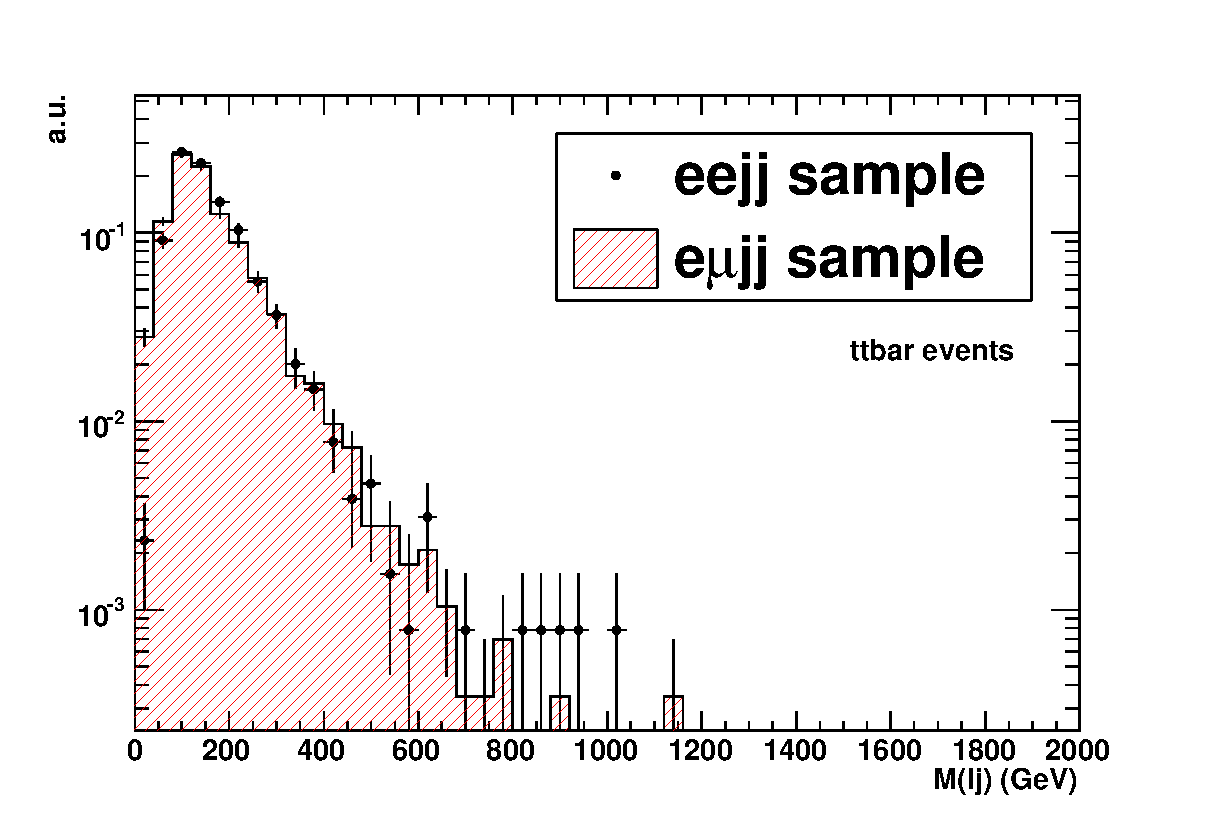
\includegraphics{plots/ttbarStudies/Mlj_eejj_VS_emujj_ttbar_STcut300.eps}} &
  \resizebox{8cm}{!}{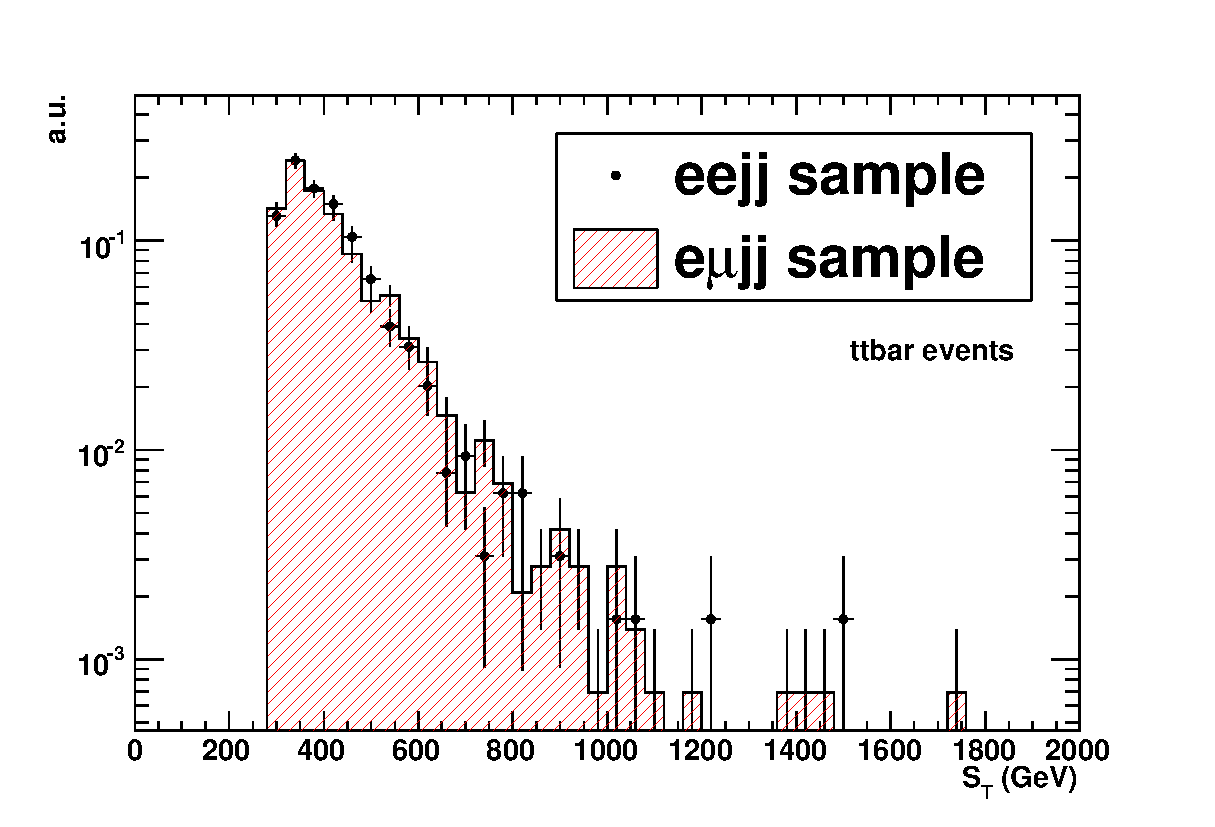
\includegraphics{plots/ttbarStudies/ST_eejj_VS_emujj_ttbar_STcut300.eps}} \\
  \end{tabular}
  \caption{\small \sl Distributions of the lepton-jet invariant mass (left) and $S_{T}$ for the eejj and the e$\mu$ samples, for $t\bar{t}$ events.
  Baseline selection criteria described in Section~\ref{sec:eventSelection} are applied, but the $S_{T}$ cut has been released to 300 GeV.}
  \label{fig:ttbar}
  \end{center}
\end{figure}

\begin{figure}[htb]
  \begin{center}
  \begin{tabular}{cc}
  \resizebox{10cm}{!}{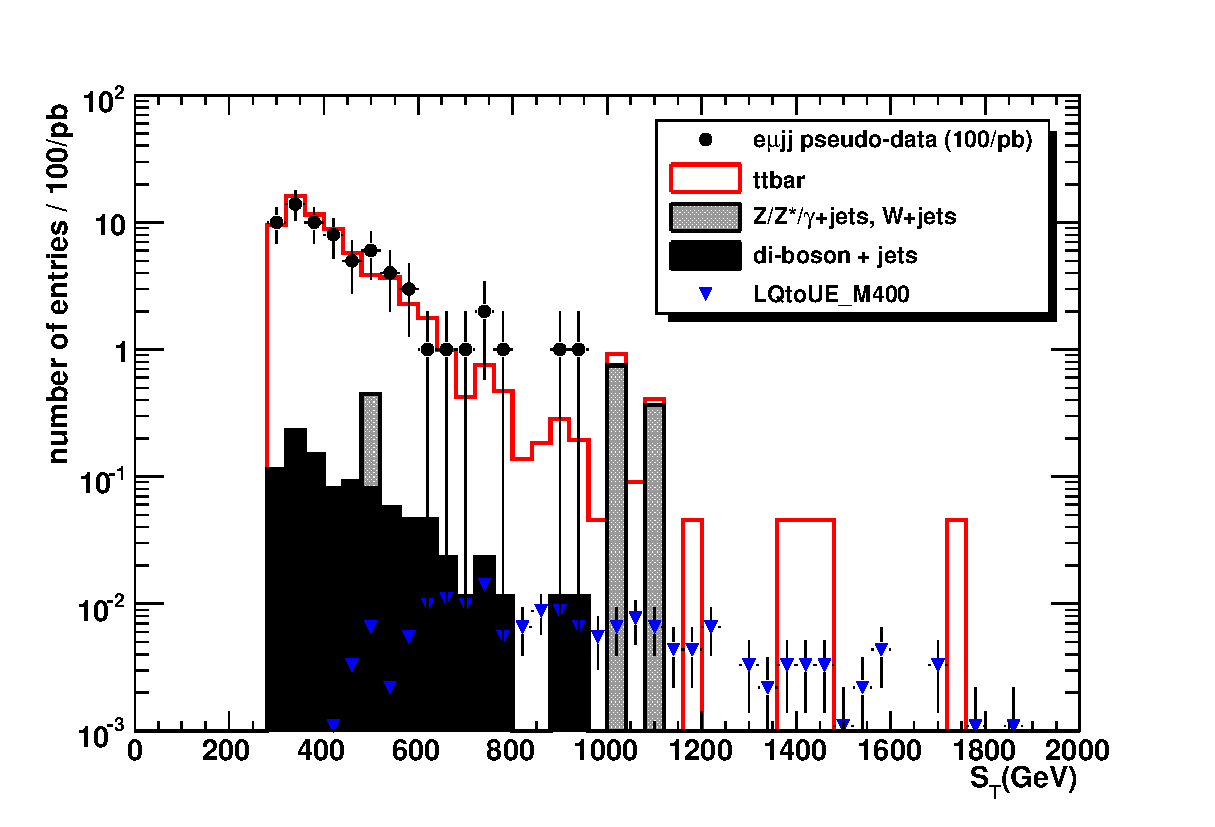
\includegraphics{plots/ttbarStudies/ST_emujj_100pb-1_STcut300.eps}} 
  \end{tabular}
  \caption{\small \sl Distribution of the $S_{T}$ variable for e$\mu$jj sample
    for different background components. 
    Histogram of signal events (at 400~GeV LQ mass) is also added. 
    Baseline selection criteria described in Section~\ref{sec:eventSelection} 
    are applied, but the $S_{T}$ cut has been released to 300 GeV.
    The background histograms are summed on top of each other.
    Black dots indicate pseudo data randomly generated accordingly with 
    the total background distribution, and assuming 100 $pb^{-1}$ of data.}
  \label{fig:emujjContamination}
  \end{center}
\end{figure}


\subsection{$Z/\gamma$+jet background shape} 

The same concept of control sample can be applied to estimate the $M_{ej}$ shape of the $Z/\gamma$+jet background.
In this case the control sample can be obtained by using the same selection criteria applied for the eejj sample except the $M_{ee}$ cut, which is modified to select events with a real $Z$ boson reconstructed ($80\mbox{ GeV} < M_{ee} < 100\mbox{ GeV}$). 
This control sample is an almost pure sample of  
$Z/\gamma$+jet events (about 4\% contamination dominated by $t\bar{t}$ and $WZ$ events) 
since the cross section of the process is resonant at the Z mass, and is 
independent from the signal sample by construction. In addition the control sample has about 10 times the number of $Z/\gamma$+jet events in 
the signal sample (about 50 events expected in the control sample for 100 pb$-1$ of data), which 
is important to reduce the statistical errors in the determination of the background shape.

Figure~\ref{fig:zjet} shows the good agreement between the shape of the $M_{ej}$ distribution for the two samples 
with the current MC statistics available. The agreement observed can be interpreted as the consequence of the 
weak correlation between the two reconstructed quantities $M_{ej}$ and $M_{ee}$ for selected events.  
%In other words it is observed that eejj events with high $M_{ej}$ are equally likely to havec high or low $M_{ee}$.

The selected events pass the cut $S_{t}>400~$GeV, which requires the presence of high $P_{T}$ electrons in the final state. 
The two most probable ways to produce high $P_{T}$ electrons in the $Z/\gamma$+jet process are 1) via the decay of a high mass (real or virtual) boson, 
or 2) because of the substantial boost of the electrons, coming from the decay of a high $P_{T}$ boson (even with low $M_{ee}$) 
which recoils from a high $P_{T}$ parton (jet). 
If the selected events were dominated by the case 1) then a strong correlation between $M_{ej}$ and $M_{ee}$ would be expected, but this is not observed.
On the contrary the selected events are dominated by the case 2), as confirmed by Figure \ref{fig:pTeePair}, which shows the $P_{T}$
distribution at generator level of the $ee$ pair (the $P_{T}$ boson distribution) for events in the control sample (low $M_{ee}$ region) and in the signal sample (high $M_{ee}$ region).
For this reason a strong correlation between $M_{ej}$ and $M_{ee}$ is not found, and this allows the use of events within the 
Z mass window as a control sample for the signal region.

\begin{figure}[htb]
  \begin{center}
  \begin{tabular}{cc}
  \resizebox{10cm}{!}{
\includegraphics{plots/UMD.eps}} \\ 
  \end{tabular}
  \caption{\small \sl Distributions of the electron-jet invariant mass for the signal eejj sample 
    (cut 1,2,3,4)
    and the control sample (cut 1,2,4 + $80\mbox{ GeV} < M_{ee} < 100\mbox{ GeV}$), for $Z/\gamma$+jet events.}
  \label{fig:zjet}
  \end{center}
\end{figure}

\begin{figure}
  \begin{center}
  \begin{tabular}{cc}
  \resizebox{10cm}{!}{
\includegraphics{plots/UMD.eps}} \\ 
  \end{tabular}
  \caption{\small \sl Distribution of the $P_{T}$ at generator level of the electron pair ($P_{T}$ of the boson) 
    for $Z/\gamma$+jet events in the signal eejj sample 
    (cut 1,2,3,4)
    and the control sample (cut 1,2,4 + $80\mbox{ GeV} < M_{ee} < 100\mbox{ GeV}$), for $Z/\gamma$+jet events.}
  \label{fig:pTeePair}
  \end{center}
\end{figure}


%http://cmssw.cvs.cern.ch/cgi-bin/cmssw.cgi/CMSSW/Configuration/CSA07Production/data/CSA07_zjet_ptjgt20_Rmatch0.7_excl.cfg?revision=1.2&view=markup

%alpgen
%zjet_0ptz100gen
%z2j_0ptz100
%njets 2
%ebeam 7000
%ih2 1  - for proton/proton collisions
%ickkw 1 - CKKW prescription for the running of alphas's in the extra gluon emission processes	
%iqopt 1 - renormalization scale
%ptjmin 20
%etajmax 5
%drjmin 0.7
%izdecmode 4

%Fit method (histogram, unbinned, function, combination...)

%\end{document}
